\begin{frame}{Preprocessing}{How can we combine all the available data in a single set?}

    \vspace{0.5cm}
    \begin{centering}
        \hspace*{-0.5cm}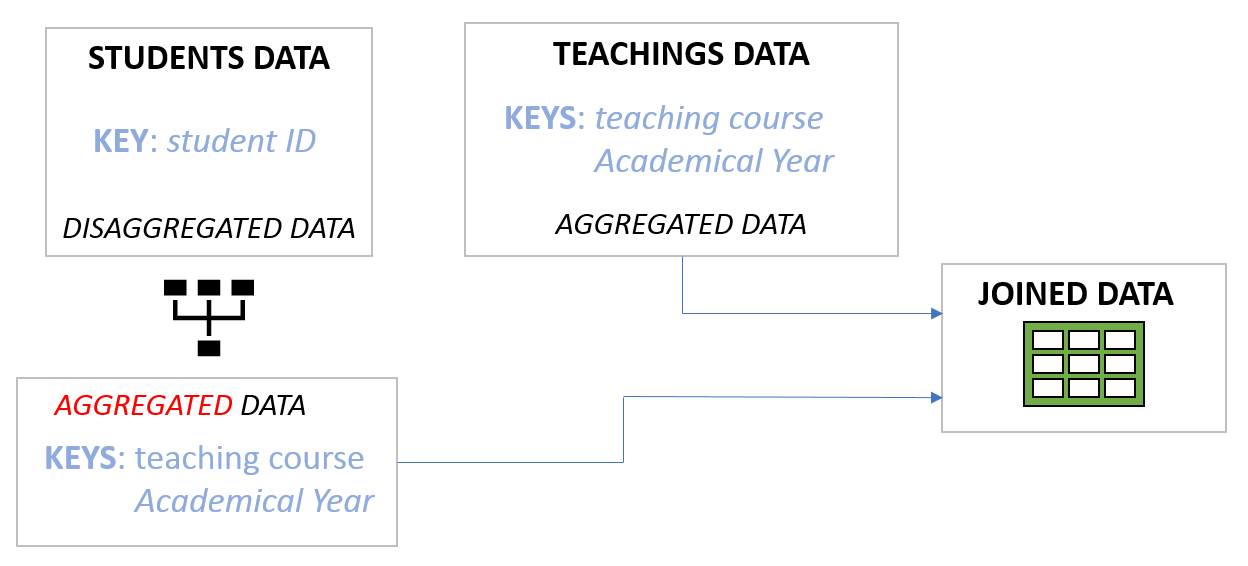
\includegraphics[scale=0.21]{img8.png}
    \end{centering}

        Raw data sets also needs \textcolor{cyan}{cleaning} --- discarding \emph{useless or redundant attributes}, \emph{invalid instances}, etc.

\end{frame}

\begin{frame}{Preprocessing}{How can we combine all the available data in a single set?}

    \alert{Example of a joined data set:}\\

    \vspace{0.35cm}

    \begin{centering}
        \hspace*{-0.65cm}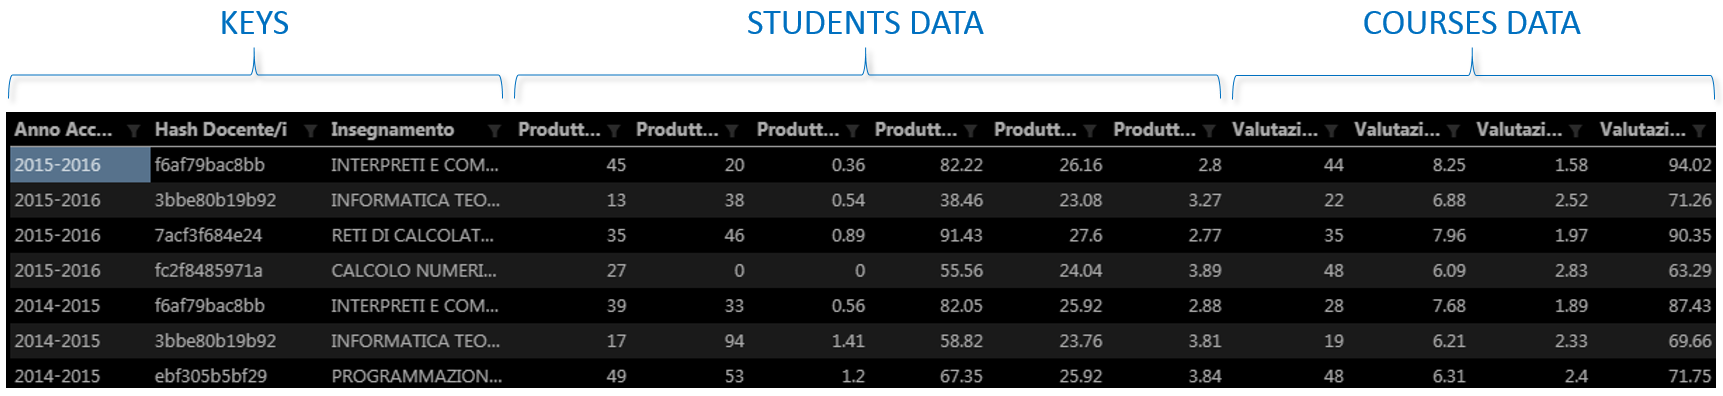
\includegraphics[scale=0.2]{prepr2.png}
    \end{centering}

    Before attemping any \emph{data mining} technique, data may still need \textcolor{cyan}{discretization}, \textcolor{cyan}{normalization}, etc. \\

 \vspace{0.5cm}

    Each analysis needs its own \emph{specific preprocessing}.

\end{frame}